\documentclass[]{article}
\usepackage{lmodern}
\usepackage{amssymb,amsmath}
\usepackage{ifxetex,ifluatex}
\usepackage{fixltx2e} % provides \textsubscript
\ifnum 0\ifxetex 1\fi\ifluatex 1\fi=0 % if pdftex
  \usepackage[T1]{fontenc}
  \usepackage[utf8]{inputenc}
  \usepackage{eurosym}
\else % if luatex or xelatex
  \ifxetex
    \usepackage{mathspec}
  \else
    \usepackage{fontspec}
  \fi
  \defaultfontfeatures{Ligatures=TeX,Scale=MatchLowercase}
  \newcommand{\euro}{€}
\fi
% use upquote if available, for straight quotes in verbatim environments
\IfFileExists{upquote.sty}{\usepackage{upquote}}{}
% use microtype if available
\IfFileExists{microtype.sty}{%
\usepackage{microtype}
\UseMicrotypeSet[protrusion]{basicmath} % disable protrusion for tt fonts
}{}
\usepackage[unicode=true]{hyperref}
\hypersetup{
            pdfborder={0 0 0},
            breaklinks=true}
\urlstyle{same}  % don't use monospace font for urls
\usepackage{graphicx,grffile}
\makeatletter
\def\maxwidth{\ifdim\Gin@nat@width>\linewidth\linewidth\else\Gin@nat@width\fi}
\def\maxheight{\ifdim\Gin@nat@height>\textheight\textheight\else\Gin@nat@height\fi}
\makeatother
% Scale images if necessary, so that they will not overflow the page
% margins by default, and it is still possible to overwrite the defaults
% using explicit options in \includegraphics[width, height, ...]{}
\setkeys{Gin}{width=\maxwidth,height=\maxheight,keepaspectratio}
\IfFileExists{parskip.sty}{%
\usepackage{parskip}
}{% else
\setlength{\parindent}{0pt}
\setlength{\parskip}{6pt plus 2pt minus 1pt}
}
\setlength{\emergencystretch}{3em}  % prevent overfull lines
\providecommand{\tightlist}{%
  \setlength{\itemsep}{0pt}\setlength{\parskip}{0pt}}
\setcounter{secnumdepth}{0}
% Redefines (sub)paragraphs to behave more like sections
\ifx\paragraph\undefined\else
\let\oldparagraph\paragraph
\renewcommand{\paragraph}[1]{\oldparagraph{#1}\mbox{}}
\fi
\ifx\subparagraph\undefined\else
\let\oldsubparagraph\subparagraph
\renewcommand{\subparagraph}[1]{\oldsubparagraph{#1}\mbox{}}
\fi

% set default figure placement to htbp
\makeatletter
\def\fps@figure{htbp}
\makeatother


\date{}

\begin{document}

23/11/2016

prof. C. Pasquarella

Infezioni correlate all'assistenza e antimicrobico-resistenza

Fabio Maestrini

sezione: Infezioni correlate all'assistenza e antimicrobico-resistenza

sottosezione: Infezioni correlate all'assistenza

Le infezioni correlate all'assistenza erano state poste dall'ECDC come
la prima minaccia per la sanità pubblica già nel 2007; nel 2008 compare
prima l'antimicromico-resistenza e successivamente le infezioni
correlate all'assistenza.

Paragrafo: \emph{Definizione}

Il termine ``infezioni correlate all'assistenza'' (ICA) ha sostituito il
termine usato da sempre

``infezioni ospedaliere'' (IO) proprio perché queste infezioni possono
essere acquisite in qualsiasi ambito in cui viene erogata assistenza
(oltre l'ospedale, assistenza ambulatoriale, case protette, residenze
assistite, ma anche l'assistenza domiciliare).

La definizione di ICA è: infezione contratta durante il processo
assistenziale, che non era presente né in incubazione al momento del
ricovero. Sono definite, infatti, comunitarie, anche quelle infezioni
che il paziente acquisisce in comunità e che poi si manifestano una
volta entrato in ospedale.

Le infezioni correlate all'assistenza si possono manifestare durante il
ricovero, ma possono emergere anche dopo la dimissione. Si pensi che
dopo interventi di artroprotesi (quindi laddove vengano impiantati
materiali estranei), le infezioni possono insorgere anche dopo un anno.
Si pensi anche a un'epatite C contratta in ambito ospedaliero: è ovvio
che può manifestarsi anche dopo la dimissione.

paragrafo: \emph{Cause}

Possono essere causate da microrganismi patogeni (che causano malattie
infettive anche in ambito comunitario) per i quali conosciamo il periodo
di incubazione, ma nella maggior parte dei casi sono causate da patogeni
opportunisti, cioè microrganismi non patogeni, ma che in caso di
immunocompromissione possono causare gravi patologie. Si riporta
l'esempio di \emph{Staphylococcus epidermidis}, che noi tutti
alberghiamo sulla cute e che può causare gravi infezioni. Per quanto
riguarda i patogeni opportunisti, si ritiene siano stati contratti in
ambito ospedaliero se l'infezione si manifesta dopo 48 ore (in alcuni
protocolli vengono indicate 24 ore, ma in genere sono 48).

L'intuizione che l'ospedale potesse essere causa di morte la ritroviamo
in questa frase del 1808 del chirurgo scozzese John Bell che dice:
``Portiamo i pazienti fuori da questa casa di morte''.

Il primo che ha oggettivato questo fenomeno è stato Ignaz Semmelweis.
Questi era un ginecologo ostetrico ungherese che, arrivato a Vienna in
un ospedale ostetrico diviso in due cliniche, osservò che queste due,
nonostante fossero adiacenti, presentavano una mortalità diversa. La
prima clinica, dove l'assistenza era operata da medici e studenti di
medicina, presentava una mortalità più che doppia rispetto alla seconda
clinica, dove l'assistenza era curata dalle ostetriche. Altre differenze
tra le due cliniche non c'erano. Semmelweis eseguì uno studio di
epidemiologia sperimentale, invertendo gli operatori sanitari: successe
che, dopo lo scambio, la mortalità risultò più elevata nella seconda
clinica, come se avesse seguito i medici e gli studenti di medicina. Il
problema, infatti, era che i medici e gli studenti, prima di andare ad
assistere le pazienti, passavano in sala settoria: trasferivano quindi
alle donne tutti gli organismi della putrefazione. Semmelweis impose il
lavaggio delle mani con cloruro di calcio: immediatamente la mortalità
delle pazienti si allineò con quella della clinica gestita dalle
ostetriche.

A Semmelweis dobbiamo l'introduzione di quella che ancora oggi è la
singola pratica più efficace per la prevenzione delle malattie infettive
trasmissibili, cioè l'igiene delle mani (che purtroppo ancora oggi trova
un' adesione scarsa).

paragrafo: \emph{Frequenza e costi}

Le infezioni correlate all'assistenza sono eventi frequenti: si stima
che dal 3 al 12\% in media i pazienti contraggano infezione, ma ci sono
reparti come la terapia intensiva dove si arriva al 30-40\%. in Italia
stimiamo tra i 450 e i 700000 pazienti con ICA, con una mortalità
attorno ai 4500-7000. In Unione Europea si stimano 4 milioni e mezzo di
infezioni con 50000 morti, negli Stati Uniti d'America 1700000 con 90000
morti. È quindi un evento frequente con un elevato impatto economico: le
stime sono di 6 miliardi all'anno negli USA, in Italia 900 milioni
all'anno.

I \textbf{costi} si possono dividere in:

\begin{itemize}
\item
  costi \textbf{ben documentati}, oggettivabili: cura delle infezioni
  (farmaci), esami diagnostici, aumento del tempo di degenza
  (quest'ultimo è il parametro utilizzato per quantificare i costi);
\item
  costi \textbf{non ben documentati}: riduzione dell'attività
  assistenziale (si pensi a quanto l'esplosione di un'epidemia in un
  reparto vada a compromettere l'attività assistenziale), cause legali,
  perdite economiche per la comunità (assenza dal lavoro per il malato e
  per chi si occupa di lui).
\end{itemize}

paragrafo: \emph{Fattori di rischio}

È documentato che le infezioni correlate all'assistenza possono essere
prevenute, quindi sono in parte evitabili con l'adozione di misure di
provata efficacia. Questa evidenza deriva da uno studio degli anni
Settanta ancora oggi valido che ha rappresentato un pilastro in questo
ambito: questo studio ha evidenziato che nel corso degli anni le
strutture dove non si mettono in atto degli interventi di provata
efficacia vedono \textbf{aumentare} queste infezioni (quindi non
rimangono stabili, vanno aumentando). Strutture che attuano interventi
di prevenzione e controllo di queste infezioni, riescono a ridurle di
una percentuale del 30\% sul totale.

Qual è il motivo dell'aumento nel primo caso? Quali sono i fattori che
incidono su questo aumento? Dagli anni Settanta a oggi è aumentata la
popolazione senile e più in generale c'è un costante aumento
dell'\textbf{immunocompromissione}. La popolazione senile è
immunocompromessa. Si pensi, però, anche ad altri casi, quali il
trapianto di midollo osseo, dove per circa una settimana il soggetto è
privo di difese: si ricordi che questi pazienti un tempo morivano. Si
pensi anche al fatto che oggi si tengono in vita neonati prematuri di
600 grammi, che un tempo morivano anche loro. Lo stesso discorso si può
fare per grandi ustionati, pazienti oncologici: tutto questo porta a un
aumento d'immunocompromissione. Ovviamente questi soggetti sono tenuti
in vita con procedure invasive.

L'immunocompromissione riguarda tutti i nostri meccanismi di difesa, a
cominciare dalla cute dove ci sono i microrganismi della flora
commensale (i commensali sono i microrganismi presenti sull'organismo
vivente, i saprofiti sono quelli presenti nell'ambiente; spesso i due
termini vengono confusi); anche la \emph{patologia di base} può
compromettere questa difesa (un trauma, un'ustione, un intervento
chirurgico).

Ci sono anche \emph{interventi iatrogeni} che vanno ad aumentare questa
compromissione. È dimostrato che un paziente cambia la sua popolazione
microbica quando viene ricoverato e acquisisce quella dell'ospedale.
Anche il \emph{trattamento antibiotico} altera e modifica la popolazione
microbica. Tutte le \emph{procedure intravascolari}, le \emph{patologie
di base del tratto respiratorio} e interventi quali \emph{intubazione},
\emph{anestesia}, \emph{broncoscopie} aumentano l'immunocompromissione.
Lo stesso discorso vale per il \emph{tratto gastrointestinale}, per le
\emph{neoplasie del sangue}, l'utilizzo di \emph{farmaci citotossici}.
Questo stato riguarda anche il complemento, l'immunità umorale e quella
cellulare.

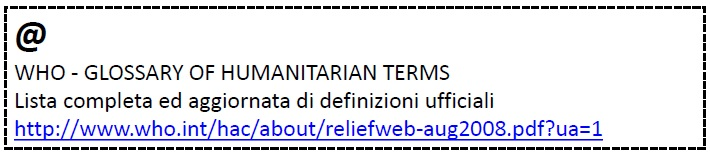
\includegraphics[width=3.48750in,height=2.69236in]{media/image1.jpeg}

Anche gli \textbf{anziani} sono immunocompromessi. Ecco tutte le
modifiche: alterazione e riduzione dei linfociti T e B,
l'assottigliamento cutaneo, compromissione di meccanismi di difesa quali
il riflesso della tosse, ma anche una riduzione delle IgA delle mucose e
una riduzione dell'acidità gastrica.

Parlando di \textbf{tecniche invasive} vediamo come la procedura sia
associata all'infezione: il \emph{cateterismo urinario} è associato a
infezione delle vie urinarie. Anche \emph{cateteri venosi e arteriosi}
non fanno altro che aprire un varco per la diffusione delle infezioni.

paragrafo: \emph{Prevenzione}

Oggi la stima delle infezioni prevenibili (da questo studio pubblicato
nel 2003) è stata allargata tra il 10 e il 70\%, soprattutto per le
infezioni del sito chirurgico. Possiamo comunque tenere che
\textbf{almeno il 30\% è prevenibile}. Ciò significa che in Italia
potremmo prevenire circa 150000 infezioni.

Rivedendo la \textbf{catena epidemiologica} delle malattie infettive,
vediamo quali sono le particolarità delle infezioni correlate
all'assistenza rispetto alle altre infezioni: riconosciamo una
\textbf{sorgente d'infezione}, l'\textbf{oggetto dell'infezione},
\textbf{veicoli e vettori}.

La \textbf{sorgente d'infezione} delle malattie infettive di comunità è
un malato o un portatore. Nelle ICA sorgente d'infezione può essere
\textbf{chiunque}: tutti noi disperdiamo organismi patogeni ma anche
opportunisti. Si veda a esempio l'apparato respiratorio: tutti noi
quando parliamo, tossiamo, starnutiamo, emettiamo le goccioline di
Flügge.


\includegraphics[width=4.07639in,height=2.45903in]{media/image2.jpeg}Le
goccioline più grandi (\emph{large droplets}, dimensioni superiori a 5
μm) sedimentano per terra nel raggio di un metro, vanno incontro a
evaporazione, ma il microrganismo rimane e può essere risollevato con la
polvere (quindi attenzione alla pulizia delle superfici). Poi abbiamo
delle goccioline più leggere (i \emph{droplet nuclei}), inferiori ai 5
μm, che invece possono essere trasportate anche a notevole distanza. Ci
sono malattie infettive, anche di comunità, che riconoscono una via di
trasmissione principale attraverso le droplet pesanti, mentre altre sono
trasmesse prevalentemente da droplet nuclei. Per esempio la trasmissione
dell'influenza è associata alle goccioline più grosse, tanto che durante
le epidemie si raccomanda una distanza di sicurezza di almeno un metro
dalla persona infetta.

Tutti noi, anche quando stiamo fermi, disperdiamo particelle. Alcuni
studi hanno dimostrato che durante un'attività (per esempio, in
palestra), sono disperse 50 milioni di particelle di dimensioni comprese
fra 0 e 3 μm. I microrganismi in genere sono veicolati da particelle di
10-20 μm; si stima che una persona in media distribuisca in un minuto
50000 microrganismi. Quindi ecco perché in sala operatoria è
raccomandato di muoversi il meno possibile e di usare i dispositivi di
protezione. Posso infatti depositare microrganismi sul camice o sul
fazzoletto, e da qui si possono poi disperdere. Oppure i microrganismi
possono sedimentare per poi essere risollevati.

A differenza delle infezioni comunitarie, nelle infezioni correlate
all'assistenza \textbf{sorgente d'infezione} può essere il
\textbf{paziente stesso}. Quindi distinguiamo ICA a \emph{sorgente
endogena} ed \emph{esogena}. Nel caso delle infezioni endogene, i
microrganismi fanno parte della popolazione microbica residente del
paziente: per esempio, \emph{Staphylococcus epidermidis} presente sulla
cute del paziente può andare a causare infezione del sito chirurgico;
\emph{Escherichia coli} va a causare un'infezione delle vie urinarie.

\textbf{Oggetto dell'infezione} è il \textbf{paziente
immunocompromesso}. Anche nel caso delle ICA c'è la \emph{possibilità di
trasmissione indiretta} attraverso dei \textbf{veicoli}: tutto ciò che
circonda il paziente può favorire la trasmissione (\emph{acqua, aria,
superfici, alimenti, dispositivi, farmaci, flaconi di disinfettante}).
Anche un \emph{operatore} può veicolare infezioni da un paziente a un
altro (se non si lava le mani e non attua misure di prevenzione).

paragrafo: \emph{Epidemiologia}

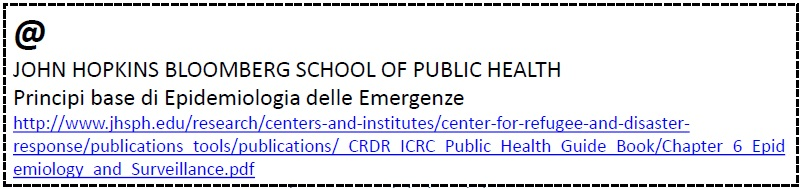
\includegraphics[width=5.00833in,height=3.53264in]{media/image3.jpeg}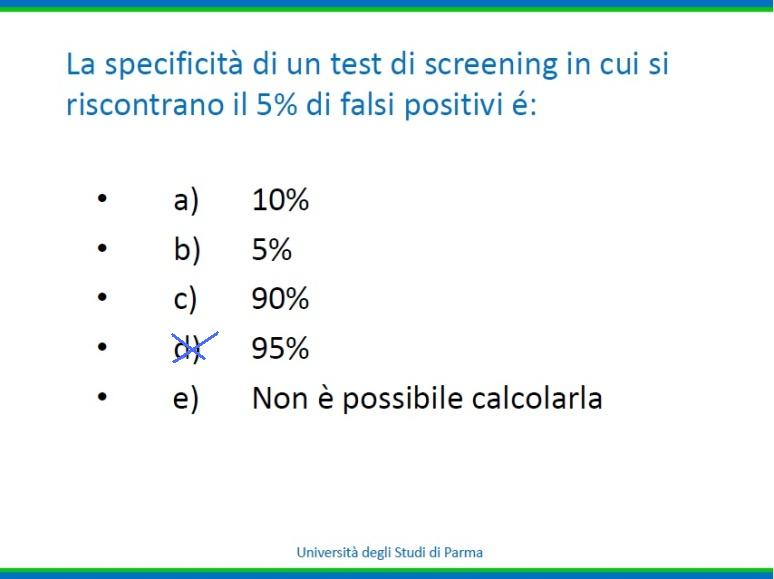
\includegraphics[width=4.98681in,height=3.58819in]{media/image4.jpeg}

Vediamo un quadro epidemiologico a livello mondiale. Vediamo la
prevalenza di ICA in paesi industrializzati: la Germania ha il 3,6\%,
mentre il Canada è a 11,6\%, l'Italia 6,7\%. Nei paesi in via di
sviluppo la prevalenza è più alta. Si ricordi che si tratta di
prevalenza, quindi non si tiene conto dell'andamento (la Germania il
mese dopo potrebbe avere il 15\%): potrebbe essere un dato non proprio
rappresentativo del fenomeno (se per coincidenza mi ritrovassi a
valutare questi dati durante un'epidemia, avrei valori altissimi). Tutti
questi studi di prevalenza peccano soprattutto di protocolli diversi e
di una mancata standardizzazione, cose che rendono molto difficile il
confronto; su questo si è lavorato, tanto che nel 2011-2012 è partito in
Europa e viene ripetuto in questi giorni il primo studio di prevalenza
standardizzato. Anche l'Italia ha partecipato, con un campione di 15000
pazienti di ospedali diversi su tutto il territorio nazionale. Da questo
studio è emerso che il 6\% dei pazienti presenta almeno un'infezione: di
questi, il 92\% ne presenta una, ma ci sono pazienti che ne presentano
due o tre. La prevalenza in Italia è risultata del 6,3\%; a livello
europeo si va dal 2,3\% della Lettonia al 10\% del Portogallo. Oltre al
dato misurato, è stato anche calcolato un dato stimato, in base al
numero di pazienti con fattori di rischio (per esempio i ricoverati in
terapia intensiva).

Relativamente al sito d'infezione, vediamo come polmoniti (infezioni
delle basse vie respiratorie), infezioni del sito chirurgico, delle vie
urinarie e del torrente ematico rappresentano circa l'80\% di tutti i
siti.

Anche in Italia troviamo questi siti nelle prime quattro posizioni in
graduatoria per frequenza. La terapia intensiva è il reparto dove si
riscontra la più alta percentuale di infezioni.

Relativamente ai microrganismi isolati a livello europeo,
\emph{Escherichia coli} ha la più alta percentuale di infezioni nelle
vie urinarie; \emph{Staphylococcus aureus}, è responsabile, invece, di
infezioni delle basse vie respiratorie e del sito chirurgico;
\emph{Pseudomonas aeruginosa} ha un'elevata percentuale per le
polmoniti. Nella nostra realtà italiana, il microrganismo più frequente
è \emph{Klebsiella}, cui seguono \emph{E. coli, Pseudomonas} e
\emph{Candida.} L'aspetto preoccupante qui è
l'\textbf{\emph{antimicrobico-resistenza}}: abbiamo addirittura
\emph{Acinetobacter baumannii} resistente per il 95\%, oltre a MRSA
(\emph{Staphylococcus aureus} meticillino-resistente) che è al 62\%
(quando in altri paesi, invece, è diminuito). Questo è oggi l'allarme.

Per chiarire i termini, antimicrobico è l'agente che va contro virus,
batteri, miceti e parassiti. Se ci si riferisce ai soli batteri, il
termine dovrebbe essere ``antibatterico'', ma viene utilizzato anche il
termine ``antibiotico''.

Sottosezione: Antimicrobico-resistenza

L'antimicrobico-resistenza (AMR) è la resistenza a un farmaco che
inizialmente era attivo. In Italia la situazione è preoccupante, una
vera emergenza. Questo sia per i gram-positivi che per i gram-negativi.
Notiamo anche resistenza ai carbapenemi, che sono considerati i farmaci
di ultima linea. L'Italia è al secondo posto dopo il Portogallo per
percentuale di resistenza di \emph{Acinetobacter} ai carbapenemi. Questi
sono i dati di prevalenza del 2011-2012. Nel 2014 il dato è addirittura
peggiorato e vediamo anche \emph{Klebsiella} resistente ai
fluorochinoloni. Il quadro è drammatico.

Paragrafo: \emph{Epidemiologia}

In un recentissimo studio sulla terapia intensiva, \emph{Acinetobacter}
resistente ai carbapenemi ha raggiunto il 97,90\%. Per alcune infezioni
non abbiamo più a disposizione farmaci.

Viene utilizzata la sigla \textbf{MDRO} (Multi Drug Resistant
Organisms): in genere la denominazione fa riferimento a un solo
antibiotico (per esempio MRSA, \emph{Staphylococcus aureus}
Meticillino-Resistente) ma la resistenza di solito è a più farmaci.

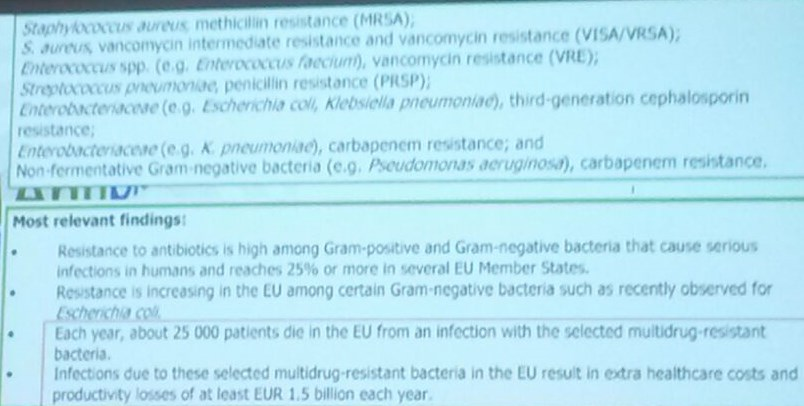
\includegraphics[width=4.27569in,height=2.15903in]{media/image5.jpeg}Per
avere un'idea della velocità di comparsa della resistenza, MRSA è stato
il primo a comparire nel 1968 negli Stati Uniti d'America. Nel 2003 la
percentuale di MRSA era del 59,5\% (sul totale di \emph{S. aureus}).
Confrontando i dati del 2002 con quelli del 2008 vediamo come i dati
siano peggiorati.

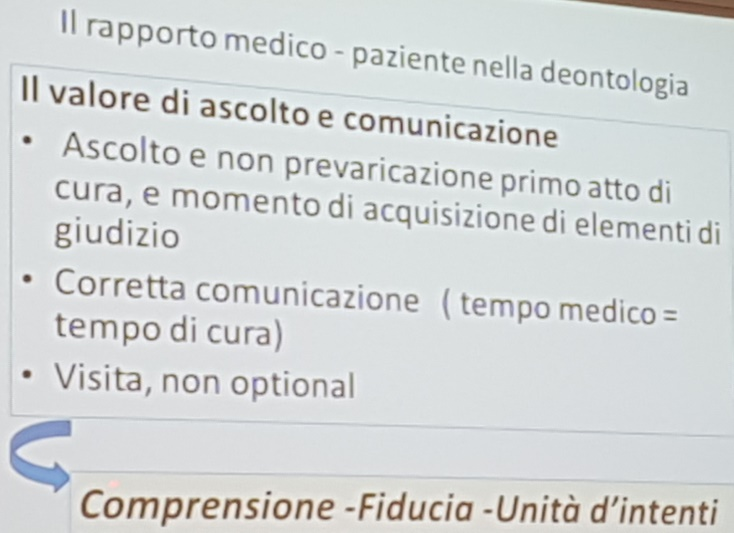
\includegraphics[width=4.40069in,height=2.67708in]{media/image6.jpeg}Oggi,
grazie a misure di controllo, la percentuale si è un po' ridotta, anche
se in Italia non così tanto come invece in altri paesi, quali a esempio
la Gran Bretagna. Il primo allarme in Europa era stato dato da questo
documento del 2009 che aveva evidenziato come ogni anno circa 25000
pazienti morissero per un'infezione da batteri multiresistenti, con un
aggravio di costi di 1,5 miliardi di lire. Il dato che è aumentato di
più è la resistenza ai gram-negativi (\emph{E. coli} resistente alle
cefalosporine di terza generazione). Oggi l'allarme è globale.

L'OMS sottolinea come non sia una fantasia quella di pensare di morire
per una ferita infetta. Ci sono stime al 2050 in cui i morti
attribuibili all'antibiotico-resistenza sono 10 milioni.

L'impatto dell'antimicrobico-resistenza sul PIL (Prodotto Interno Lordo)
arriva a pesare per milioni di dollari.

Le \textbf{conseguenze} facilmente intuibili:

\begin{itemize}
\item
  trattamenti più difficili oppure nessun trattamento disponibile,
\item
  ritardo nel trattamento,
\item
  impossibilità a somministrare una terapia,
\item
  prolungamento inevitabile della degenza, con tutti i rischi che
  comporta,
\item
  aumento di complicanze,
\item
  aumento della mortalità,
\item
  aumento dei costi, per diagnosi, terapia e degenza.
\end{itemize}

Vediamo a esempio come la mortalità per MRSA sia del 21\%, contro l'8\%
delle infezioni da MSSA (\emph{S. aureus} suscettibile alla
meticillina). Il costo nel primo caso è aumentato del 22\%.

Ci si sta muovendo da più parti a livello globale e per la quarta volta
nella storia delle nazioni unite, il 21 settembre 2016 è stata discussa
l'antimicrobico-resistenza. L'OMS ha disposto un piano di azione
globale, così come l'Europa. Anche il Ministero della Salute ha
predisposto un piano di contrasto 2017-2020, che si spera venga
pubblicato entro la fine del 2016.

paragrafo: \emph{Cause}

L'antimicrobico-resistenza è un fenomeno naturale. Ci potrebbe essere
una \emph{mutazione spontanea} oppure l'\emph{acquisizione di materiale
genetico}, ma sicuramente è un fenomeno accelerato
dall'\emph{\textbf{uso inappropriato di antibiotici} sia nell'uomo che
nell'ambito veterinario}.

Purtroppo sugli animali gli antibiotici vengono anche utilizzati come
fattori di crescita.

Uso inappropriato degli antibiotici comprende l'\emph{uso non
necessario} (tipico esempio è l'impiego nelle malattie virali), ma anche
\emph{dosaggi inappropriati}, \emph{interruzione della terapia prima del
termine raccomandato}.

Questi sono dati di antibiotici prescritti senza reale necessità: si
notino antibiotici usati erroneamente per influenza e raffreddore. È un
fenomeno che in Italia è comune su tutto il territorio nazionale agli
stessi livelli. Ci sono casi di antibiotici somministrati in ritardo e
casi di utilizzo di antibiotici a largo spettro (quando invece la
terapia deve essere mirata). A volte il trattamento è troppo breve o
troppo lungo, oppure non basato sul risultato dell'antibiogramma.

Si noti il caso della \emph{\emph{profilassi antibiotica in chirurgia}},
che è uno di quegli ambiti in cui maggiore è il divario tra quanto
raccomandato in letteratura e quanto in realtà effettuato. Ci sono
infatti \emph{linee guida} ben precise per ogni intervento, con
l'indicazione del farmaco di elezione (che nella maggior parte dei casi
è una cefalosporina di prima generazione), la dose, il momento di
somministrazione (il farmaco deve essere efficace al momento
dell'intervento, non troppo presto, per il rischio d'infezione da
\emph{Clostridium difficile}), la durata (nella maggior parte dei casi
basta una sola dose di antibiotico, o al massimo la si può prolungare
per 24 ore dopo l'intervento).

Gl'interventi sono classificati in puliti, puliti-contaminati,
contaminati e sporchi, a seconda della presenza dei microrganismi nel
sito d'infezione.

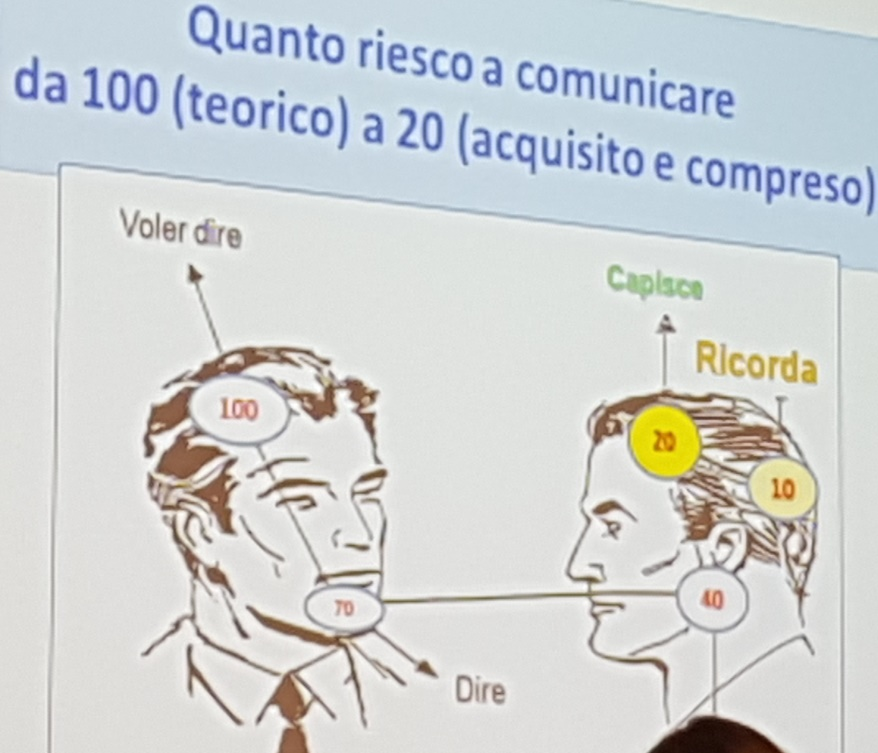
\includegraphics[width=3.43472in,height=3.00556in]{media/image7.jpeg}Quindi
\textbf{interventi puliti} sono quelli in cui si opera su siti
``sterili'' (cioè se l'antisepsi è effettuata correttamente,
microrganismi non ci sono): è il caso di interventi di ortopedia, di
chirurgia vascolare. In questi \emph{interventi puliti l'antibiotico non
dovrebbe essere somministrato} (a meno che non si impianti materiale
protesico). L'evidenza scientifica dimostra che nella chirurgia pulita
la somministrazione dell'antibiotico è inutile. L'antibiotico deve
essere somministrato entro 30-60 minuti al massimo prima
dell'intervento, perché in questo modo il farmaco è presente durante
l'intervento e ha la maggiore efficacia.


\includegraphics[width=3.75694in,height=2.80347in]{media/image8.jpeg}

Vediamo questo studio in cui vengono elencati i casi di \textbf{utilizzo
inappropriato di antibiotici}. Nel 74\% degli interventi puliti è stata
somministrata profilassi antibiotica. Nel 40\% dei casi la profilassi è
durata più di 24 ore. Ci sono casi in cui la profilassi è stata iniziata
addirittura dopo l'intervento, quando non ha alcun senso. La corretta
somministrazione antibiotica è all'induzione, quindi al momento
dell'anestesia, tant'è che il responsabile della somministrazione
dell'antibiotico dovrebbe essere l'anestesista.

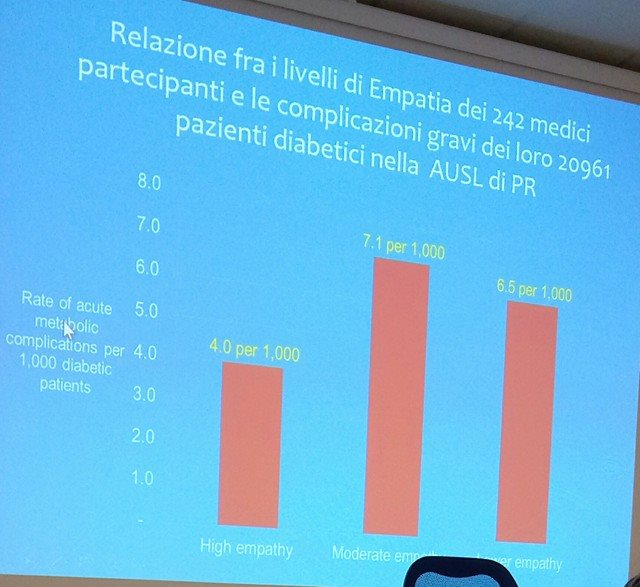
\includegraphics[width=3.15278in,height=1.94167in]{media/image9.jpeg}

In questo studio si vede come addirittura a volte la profilassi
antibiotica duri giorni; sono stati valutati i costi: in tre mesi sono
stati spesi 26000\euro{}, a fronte dei 3000\euro{} spesi seguendo le
linee guida. Il problema, comunque non è solo italiano.

A proposito di linee guida, bisogna anche considerare le resistenze
locali: se la percentuale di MRSA nella struttura è superiore al 50\%,
invece della cefazolina di prima generazione si può usare la
vancomicina. Bisogna anche considerare eventuali allergie del paziente.

Per quanto riguarda il consumo di antibiotici in ambito
extra-ospedaliero, l'Italia ha livelli molto alti. A livello globale
l'Italia è al secondo posto per uso inappropriato dopo la Grecia.

Fra il 2000 e il 2010 il consumo nel mondo è aumentato del 36\%: fra i
paesi in cui l'aumento è stato maggiore ci sono Brasile, Russia, India
(dove le resistenze sono le più alte al mondo), Cina (addirittura del
76\%). C'è stato un aumento di consumo di carbapenemi e polimixina, che
sono l'ultima riserva.

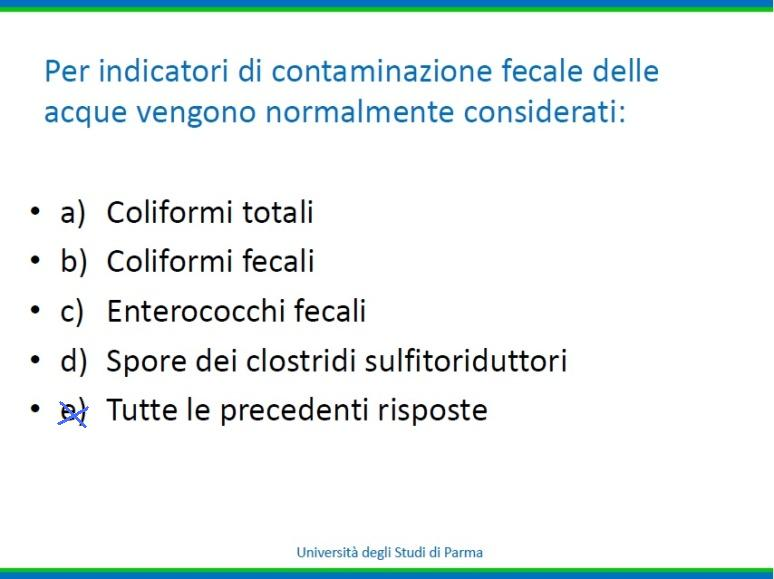
\includegraphics[width=3.68056in,height=1.90347in]{media/image10.jpeg}Ricordiamo
anche i problemi legati alla scarsa igiene, alla scarsa ricerca di nuovi
antibiotici e all'uso in ambito veterinario. Gli animali vengono
trattati in modo eccessivo con antibiotici e veicolano batteri
resistenti, che arrivano agli ortaggi (terreno concimato con letame) e
all'uomo.

Nelle \textbf{strutture sanitarie} c'è una diffusione molto facile
\emph{dall'operatore al paziente}, ma anche \emph{tra paziente e
paziente} e \emph{tra visitatori e degenti} (e viceversa: lavarsi le
mani prima di lasciare l'ospedale). Poi c'è anche la globalizzazione: di
ritorno da un viaggio si possono acquisire microrganismi resistenti, non
necessariamente dopo essere passati in un ospedale straniero, ma anche
per una contaminazione del cibo. Oggi si parla di \textbf{ONE HEALTH}:
la salute è una, in ambito veterinario e umano.

Paragrafo: \emph{Misure da attuare}

Ognuno deve fare la sua parte. Un \textbf{operatore} deve senza dubbio:

prevenire le infezioni, anche attraverso le vaccinazioni

uso appropriato di antibiotico e raccomandazione al paziente.

\subsection{\texorpdfstring{Il \textbf{paziente}
deve:}{Il paziente deve:}}\label{il-paziente-deve}

\begin{itemize}
\item ~
  \subsection{usare l'antibiotico solo quando prescritto dal
  medico}\label{usare-lantibiotico-solo-quando-prescritto-dal-medico}
\item ~
  \subsection{effettuare correttamente la terapia per la sua intera
  durata}\label{effettuare-correttamente-la-terapia-per-la-sua-intera-durata}
\item ~
  \subsection{mai condividere l'antibiotico con altri che hanno gli
  stessi
  sintomi}\label{mai-condividere-lantibiotico-con-altri-che-hanno-gli-stessi-sintomi}
\item ~
  \subsection{prevenire le infezioni}\label{prevenire-le-infezioni}
\end{itemize}

\subsection{\texorpdfstring{Le \textbf{istituzioni}, da parte loro,
devono:}{Le istituzioni, da parte loro, devono:}}\label{le-istituzioni-da-parte-loro-devono}

\begin{itemize}
\item ~
  \subsection{muoversi con piani di
  azione}\label{muoversi-con-piani-di-azione}
\item ~
  \subsection{migliorare la
  sorveglianza}\label{migliorare-la-sorveglianza}
\item ~
  \subsection{rafforzare la prevenzione e il
  controllo}\label{rafforzare-la-prevenzione-e-il-controllo}
\item ~
  \subsection{diffondere le informazioni
  sull'antibiotico-resistenza.}\label{diffondere-le-informazioni-sullantibiotico-resistenza.}
\end{itemize}

\subsection{\texorpdfstring{Nel \textbf{settore veterinario}
bisogna:}{Nel settore veterinario bisogna:}}\label{nel-settore-veterinario-bisogna}

\begin{itemize}
\item ~
  \subsection{utilizzare l'antibiotico solo per trattare le
  infezioni}\label{utilizzare-lantibiotico-solo-per-trattare-le-infezioni}
\item ~
  \subsection{vaccinare gli animali}\label{vaccinare-gli-animali}
\item ~
  \subsection{regolamentare la
  produzione}\label{regolamentare-la-produzione}
\item ~
  \subsection{migliorare l'igiene}\label{migliorare-ligiene}
\item ~
  \subsection{implementare i rapporti con le
  istituzioni.}\label{implementare-i-rapporti-con-le-istituzioni.}
\end{itemize}

\subsection{Questo è il piano d'azione della commissione
europea:}\label{questo-uxe8-il-piano-dazione-della-commissione-europea}

\begin{itemize}
\item ~
  \subsection{garantire un uso adeguato degli
  antibiotici}\label{garantire-un-uso-adeguato-degli-antibiotici}
\item ~
  \subsection{prevenire le infezioni}\label{prevenire-le-infezioni-1}
\item ~
  \subsection{promuovere la ricerca e
  l'innovazione}\label{promuovere-la-ricerca-e-linnovazione}
\item ~
  \subsection{collaborare con i partner internazionali per contenere i
  rischi}\label{collaborare-con-i-partner-internazionali-per-contenere-i-rischi}
\item ~
  \subsection{migliorare il
  monitoraggio.}\label{migliorare-il-monitoraggio.}
\end{itemize}

\subsection{\texorpdfstring{È stata promossa la \textbf{Giornata europea
della Consapevolezza}, il 18 novembre di ogni anno. C'è il sito internet
con materiale disponibile in tutte le lingue. Nel 2016, anno della
sedicesima edizione, ha ricevuto lo European health
award.}{È stata promossa la Giornata europea della Consapevolezza, il 18 novembre di ogni anno. C'è il sito internet con materiale disponibile in tutte le lingue. Nel 2016, anno della sedicesima edizione, ha ricevuto lo European health award.}}\label{uxe8-stata-promossa-la-giornata-europea-della-consapevolezza-il-18-novembre-di-ogni-anno.-cuxe8-il-sito-internet-con-materiale-disponibile-in-tutte-le-lingue.-nel-2016-anno-della-sedicesima-edizione-ha-ricevuto-lo-european-health-award.}

\subsection{}\label{section}

\subsection{}\label{section-1}

\subsection{}\label{section-2}

\subsection{}\label{section-3}

\subsection{sottosezione: Prevenzione di ICA e
AMR}\label{sottosezione-prevenzione-di-ica-e-amr}

\subsection{}\label{section-4}

\subsection{Vediamo ora quali sono i cardini della prevenzione delle
infezioni correlate all'assistenza e dell'antimicrobico
resistenza:}\label{vediamo-ora-quali-sono-i-cardini-della-prevenzione-delle-infezioni-correlate-allassistenza-e-dellantimicrobico-resistenza}

\begin{enumerate}
\def\labelenumi{\arabic{enumi}.}
\item ~
  \subsection{\texorpdfstring{l'istituzione di un \textbf{comitato di
  controllo delle infezioni} (con un gruppo operativo), raccomandata già
  nel 1985 dal ministero, ma nel 2001 non si erano fatti molti passi
  avanti (soprattutto al sud); spesso questi comitati sono stati
  costituiti sulla carta ma non hanno mai lavorato (un comitato si
  ritiene attivo se si riunisce almeno quattro volte l'anno); i compiti
  del comitato
  sono:}{l'istituzione di un comitato di controllo delle infezioni (con un gruppo operativo), raccomandata già nel 1985 dal ministero, ma nel 2001 non si erano fatti molti passi avanti (soprattutto al sud); spesso questi comitati sono stati costituiti sulla carta ma non hanno mai lavorato (un comitato si ritiene attivo se si riunisce almeno quattro volte l'anno); i compiti del comitato sono:}}\label{listituzione-di-un-comitato-di-controllo-delle-infezioni-con-un-gruppo-operativo-raccomandata-giuxe0-nel-1985-dal-ministero-ma-nel-2001-non-si-erano-fatti-molti-passi-avanti-soprattutto-al-sud-spesso-questi-comitati-sono-stati-costituiti-sulla-carta-ma-non-hanno-mai-lavorato-un-comitato-si-ritiene-attivo-se-si-riunisce-almeno-quattro-volte-lanno-i-compiti-del-comitato-sono}

  \begin{itemize}
  \item ~
    \subsection{definire la strategia di
    lotta}\label{definire-la-strategia-di-lotta}
  \item ~
    \subsection{verificare l'applicazione dei programmi di
    sorveglianza}\label{verificare-lapplicazione-dei-programmi-di-sorveglianza}
  \item ~
    \subsection{curare la formazione (che deve cominciare nei corsi di
    laurea);}\label{curare-la-formazione-che-deve-cominciare-nei-corsi-di-laurea}
  \end{itemize}
\end{enumerate}

\subsection{\texorpdfstring{\protect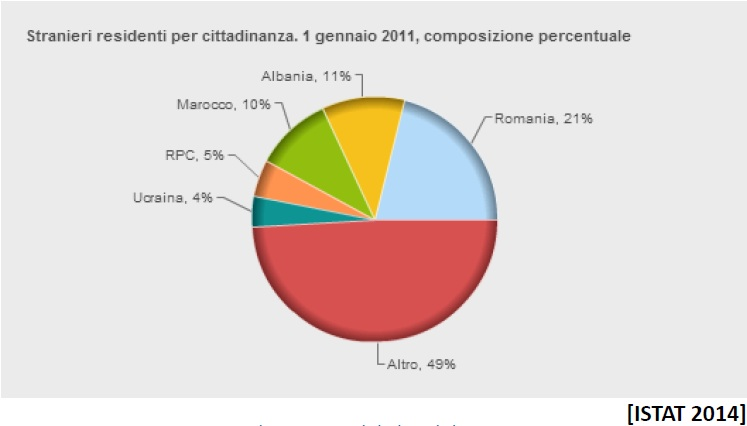
\includegraphics[width=2.43819in,height=1.55069in]{media/image11.jpeg}}{}}\label{section-5}

\begin{enumerate}
\def\labelenumi{\arabic{enumi}.}
\item ~
  \subsection{\texorpdfstring{\textbf{sorveglianza epidemiologica},
  perché l'epidemiologia è lo strumento di conoscenza per intervenire;
  quindi occorre una raccolta di dati per oggettivare il problema, come
  base per l'intervento (gli studi non sono fatti per essere tenuti nei
  cassetti); serve anche per valutare l'efficacia delle misure
  d'intervento. Peter Drucker, padre del management, diceva: ``Se non
  riesci a misurare una situazione, non la puoi gestire''. Oggi a
  livello europeo e nazionale c'è una rete di sorveglianza
  dell'incidenza per quanto riguarda la terapia intensiva e le infezioni
  del sito chirurgico. C'è poi una \emph{sorveglianza specifica per
  l'antimicrobico-resistenza} e poi una \emph{per il consumo degli
  antibiotici}.}{sorveglianza epidemiologica, perché l'epidemiologia è lo strumento di conoscenza per intervenire; quindi occorre una raccolta di dati per oggettivare il problema, come base per l'intervento (gli studi non sono fatti per essere tenuti nei cassetti); serve anche per valutare l'efficacia delle misure d'intervento. Peter Drucker, padre del management, diceva: ``Se non riesci a misurare una situazione, non la puoi gestire''. Oggi a livello europeo e nazionale c'è una rete di sorveglianza dell'incidenza per quanto riguarda la terapia intensiva e le infezioni del sito chirurgico. C'è poi una sorveglianza specifica per l'antimicrobico-resistenza e poi una per il consumo degli antibiotici.}}\label{sorveglianza-epidemiologica-perchuxe9-lepidemiologia-uxe8-lo-strumento-di-conoscenza-per-intervenire-quindi-occorre-una-raccolta-di-dati-per-oggettivare-il-problema-come-base-per-lintervento-gli-studi-non-sono-fatti-per-essere-tenuti-nei-cassetti-serve-anche-per-valutare-lefficacia-delle-misure-dintervento.-peter-drucker-padre-del-management-diceva-se-non-riesci-a-misurare-una-situazione-non-la-puoi-gestire.-oggi-a-livello-europeo-e-nazionale-cuxe8-una-rete-di-sorveglianza-dellincidenza-per-quanto-riguarda-la-terapia-intensiva-e-le-infezioni-del-sito-chirurgico.-cuxe8-poi-una-sorveglianza-specifica-per-lantimicrobico-resistenza-e-poi-una-per-il-consumo-degli-antibiotici.}
\item ~
  \subsection{\texorpdfstring{Adesioni alle \textbf{precauzioni
  standard}, ossia procedure che vanno rispettate in qualsiasi occasione
  di rapporto con il paziente: tutti i pazienti devono essere
  considerati potenzialmente
  infettanti.}{Adesioni alle precauzioni standard, ossia procedure che vanno rispettate in qualsiasi occasione di rapporto con il paziente: tutti i pazienti devono essere considerati potenzialmente infettanti.}}\label{adesioni-alle-precauzioni-standard-ossia-procedure-che-vanno-rispettate-in-qualsiasi-occasione-di-rapporto-con-il-paziente-tutti-i-pazienti-devono-essere-considerati-potenzialmente-infettanti.}

  \begin{enumerate}
  \def\labelenumii{\arabic{enumii}.}
  \item ~
    \subsection{\texorpdfstring{\textbf{Igiene delle
    mani}}{Igiene delle mani}}\label{igiene-delle-mani}
  \item ~
    \subsection{utilizzo dei
    dispositivi}\label{utilizzo-dei-dispositivi}
  \item ~
    \subsection{\texorpdfstring{sanificazione ambientale (pulizia delle
    \textbf{superfici}, sterilizzazione degli strumenti, gestioni della
    biancheria).}{sanificazione ambientale (pulizia delle superfici, sterilizzazione degli strumenti, gestioni della biancheria).}}\label{sanificazione-ambientale-pulizia-delle-superfici-sterilizzazione-degli-strumenti-gestioni-della-biancheria.}
  \end{enumerate}
\end{enumerate}

\subsection{\texorpdfstring{\protect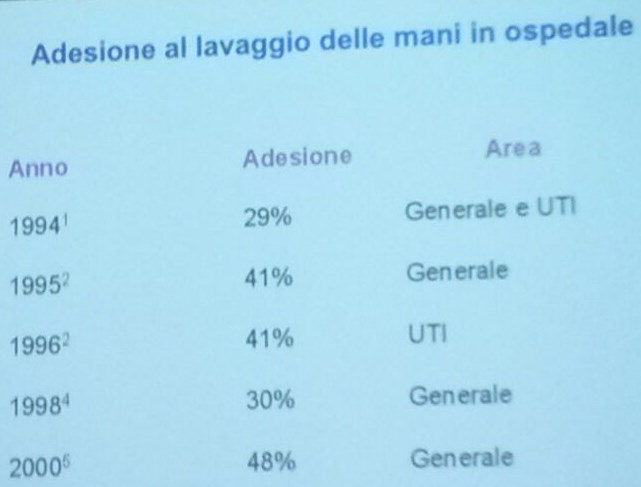
\includegraphics[width=2.97917in,height=2.26319in]{media/image12.jpeg}Purtroppo
l'adesione alla misura di igiene delle mani è ancora molto scarsa: nel
2000 in terapia intensiva l'adesione era del 40\%.
}{Purtroppo l'adesione alla misura di igiene delle mani è ancora molto scarsa: nel 2000 in terapia intensiva l'adesione era del 40\%. }}\label{purtroppo-ladesione-alla-misura-di-igiene-delle-mani-uxe8-ancora-molto-scarsa-nel-2000-in-terapia-intensiva-ladesione-era-del-40.}

\subsection{\texorpdfstring{L'OMS ha deciso di avviare una campagna dal
titolo ``Cure pulite sono cure più sicure'', promuovendo in modo
specifico il \textbf{lavaggio delle mani}. C'è una \textbf{linea guida
specifica}, con i \emph{cinque momenti} dell'igiene delle
mani:}{L'OMS ha deciso di avviare una campagna dal titolo ``Cure pulite sono cure più sicure'', promuovendo in modo specifico il lavaggio delle mani. C'è una linea guida specifica, con i cinque momenti dell'igiene delle mani:}}\label{loms-ha-deciso-di-avviare-una-campagna-dal-titolo-cure-pulite-sono-cure-piuxf9-sicure-promuovendo-in-modo-specifico-il-lavaggio-delle-mani.-cuxe8-una-linea-guida-specifica-con-i-cinque-momenti-delligiene-delle-mani}

\begin{itemize}
\item ~
  \subsection{prima del contatto con il
  paziente}\label{prima-del-contatto-con-il-paziente}
\item ~
  \subsection{prima di una manovra
  asettica}\label{prima-di-una-manovra-asettica}
\item ~
  \subsection{dopo il contatto con il paziente, per evitare di
  trasferire sulle superfici, ad altri pazienti i microrganismi
  acquisiti}\label{dopo-il-contatto-con-il-paziente-per-evitare-di-trasferire-sulle-superfici-ad-altri-pazienti-i-microrganismi-acquisiti}
\item ~
  \subsection{dopo il contatto con ciò che è attorno al paziente (tutte
  le superfici sono contaminate, come le sponde del letto, i vassoi, i
  tavolini)}\label{dopo-il-contatto-con-ciuxf2-che-uxe8-attorno-al-paziente-tutte-le-superfici-sono-contaminate-come-le-sponde-del-letto-i-vassoi-i-tavolini}
\item ~
  \subsection{dopo esposizione a qualsiasi liquido
  biologico.}\label{dopo-esposizione-a-qualsiasi-liquido-biologico.}
\end{itemize}

\subsection{\texorpdfstring{Importante è anche il come lavarsi le mani:
attenzione al palmo della mano (spesso trascurato), gli spazi
interdigitali, i polpastrelli. Fare inoltre attenzione a non chiudere il
rubinetto con le mani appena lavate. Il tempo previsto è di \emph{40
secondi}, perché l'evidenza scientifica ha dimostrato che così si ha una
riduzione significativa di
microrganismi.}{Importante è anche il come lavarsi le mani: attenzione al palmo della mano (spesso trascurato), gli spazi interdigitali, i polpastrelli. Fare inoltre attenzione a non chiudere il rubinetto con le mani appena lavate. Il tempo previsto è di 40 secondi, perché l'evidenza scientifica ha dimostrato che così si ha una riduzione significativa di microrganismi.}}\label{importante-uxe8-anche-il-come-lavarsi-le-mani-attenzione-al-palmo-della-mano-spesso-trascurato-gli-spazi-interdigitali-i-polpastrelli.-fare-inoltre-attenzione-a-non-chiudere-il-rubinetto-con-le-mani-appena-lavate.-il-tempo-previsto-uxe8-di-40-secondi-perchuxe9-levidenza-scientifica-ha-dimostrato-che-cosuxec-si-ha-una-riduzione-significativa-di-microrganismi.}

\subsection{Per promuovere l'igiene delle mani dove non c'è un
lavandino, si può usare il gel idroalcolico. In questo caso il tempo
sufficiente è di 25 secondi, ma l'attenzione a tutte le parti della mano
è ancora
fondamentale.}\label{per-promuovere-ligiene-delle-mani-dove-non-cuxe8-un-lavandino-si-puuxf2-usare-il-gel-idroalcolico.-in-questo-caso-il-tempo-sufficiente-uxe8-di-25-secondi-ma-lattenzione-a-tutte-le-parti-della-mano-uxe8-ancora-fondamentale.}

\subsection{\texorpdfstring{\protect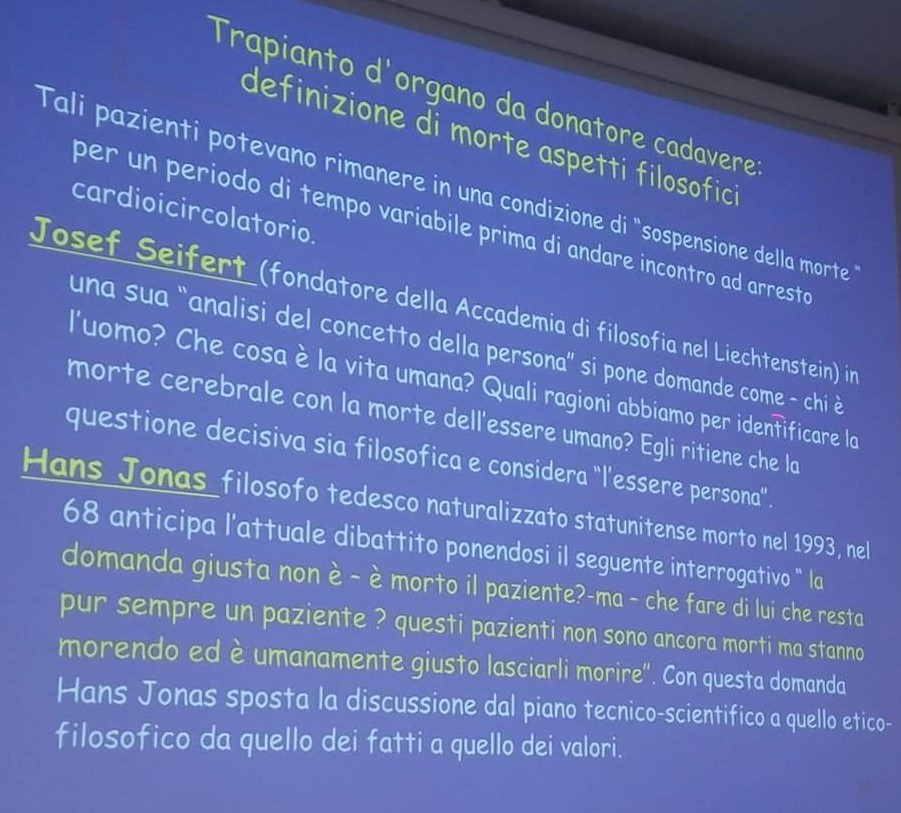
\includegraphics[width=3.86667in,height=3.05903in]{media/image13.jpeg}Oltre
all'igiene delle mani è fondamentale quella delle superfici.
}{Oltre all'igiene delle mani è fondamentale quella delle superfici. }}\label{oltre-alligiene-delle-mani-uxe8-fondamentale-quella-delle-superfici.}

\begin{enumerate}
\def\labelenumi{\arabic{enumi}.}
\setcounter{enumi}{3}
\item ~
  \subsection{Razionale uso degli
  antibiotici}\label{razionale-uso-degli-antibiotici}
\item ~
  \subsection{\texorpdfstring{\textbf{Linee guida} e \textbf{protocolli
  di
  comportamento}}{Linee guida e protocolli di comportamento}}\label{linee-guida-e-protocolli-di-comportamento}
\item ~
  \subsection{\texorpdfstring{Adeguata \textbf{progettazione della
  struttura}: lontananza dal traffico, camere d'isolamento, accessi
  appropriati per il lavaggio delle mani (spesso sono distanti),
  personale numericamente adeguato (che abbia tempo per lavarsi le mani:
  si è visto che se si è in pochi e si ha poco tempo, non ci si lava le
  mani). Ci sono anche alcune religioni che vietano di uccidere
  organismi viventi e quindi di utilizzare il gel
  idroalcolico.}{Adeguata progettazione della struttura: lontananza dal traffico, camere d'isolamento, accessi appropriati per il lavaggio delle mani (spesso sono distanti), personale numericamente adeguato (che abbia tempo per lavarsi le mani: si è visto che se si è in pochi e si ha poco tempo, non ci si lava le mani). Ci sono anche alcune religioni che vietano di uccidere organismi viventi e quindi di utilizzare il gel idroalcolico.}}\label{adeguata-progettazione-della-struttura-lontananza-dal-traffico-camere-disolamento-accessi-appropriati-per-il-lavaggio-delle-mani-spesso-sono-distanti-personale-numericamente-adeguato-che-abbia-tempo-per-lavarsi-le-mani-si-uxe8-visto-che-se-si-uxe8-in-pochi-e-si-ha-poco-tempo-non-ci-si-lava-le-mani.-ci-sono-anche-alcune-religioni-che-vietano-di-uccidere-organismi-viventi-e-quindi-di-utilizzare-il-gel-idroalcolico.}
\end{enumerate}

\subsection{\texorpdfstring{\protect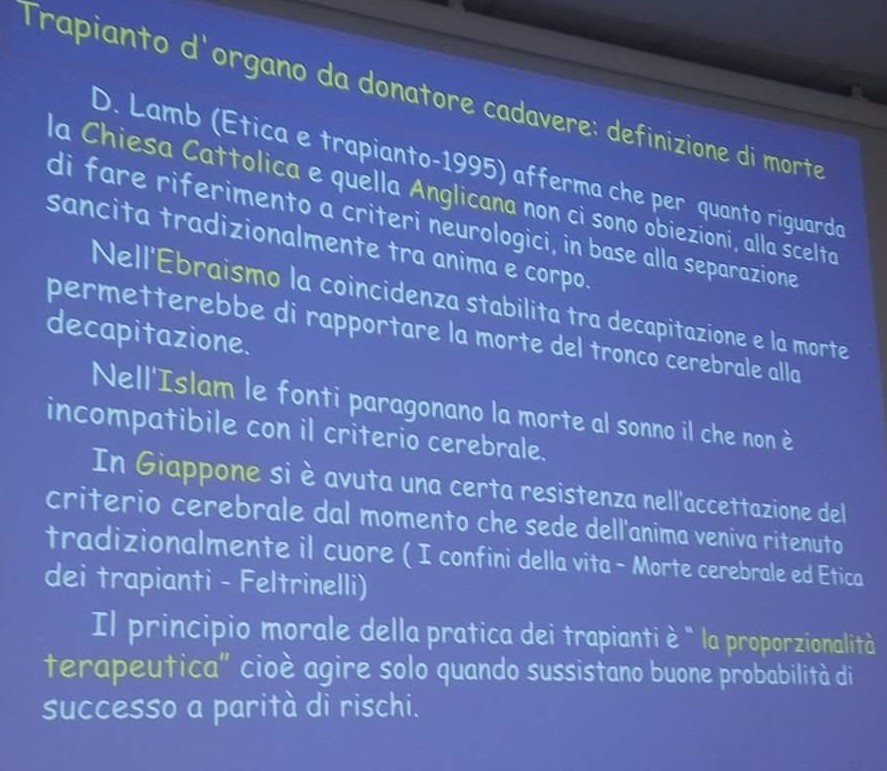
\includegraphics[width=4.43958in,height=2.85625in]{media/image14.jpeg}}{}}\label{section-6}

\subsection{\texorpdfstring{Pittet nel 2004 ha individuato i
\emph{determinanti importanti}: l'\emph{epidemiologia}, la
\emph{microbiologia} e il
\emph{comportamento}.}{Pittet nel 2004 ha individuato i determinanti importanti: l'epidemiologia, la microbiologia e il comportamento.}}\label{pittet-nel-2004-ha-individuato-i-determinanti-importanti-lepidemiologia-la-microbiologia-e-il-comportamento.}

\subsection{\texorpdfstring{Oggi c'è un aumentata evidenza del ruolo
delle superfici, soprattutto per i microrganismi multiresistenti. Le
\textbf{superfici} hanno un ruolo perché gli operatori non rispettano
l'igiene delle mani. Tutte le superfici sono contaminate:
\emph{Enterococcus} è stato trovato sulle sponde dei letti, sulle
maniglie delle porte, sugli interruttori (frequently touched
surfaces).}{Oggi c'è un aumentata evidenza del ruolo delle superfici, soprattutto per i microrganismi multiresistenti. Le superfici hanno un ruolo perché gli operatori non rispettano l'igiene delle mani. Tutte le superfici sono contaminate: Enterococcus è stato trovato sulle sponde dei letti, sulle maniglie delle porte, sugli interruttori (frequently touched surfaces).}}\label{oggi-cuxe8-un-aumentata-evidenza-del-ruolo-delle-superfici-soprattutto-per-i-microrganismi-multiresistenti.-le-superfici-hanno-un-ruolo-perchuxe9-gli-operatori-non-rispettano-ligiene-delle-mani.-tutte-le-superfici-sono-contaminate-enterococcus-uxe8-stato-trovato-sulle-sponde-dei-letti-sulle-maniglie-delle-porte-sugli-interruttori-frequently-touched-surfaces.}

\subsection{\texorpdfstring{\protect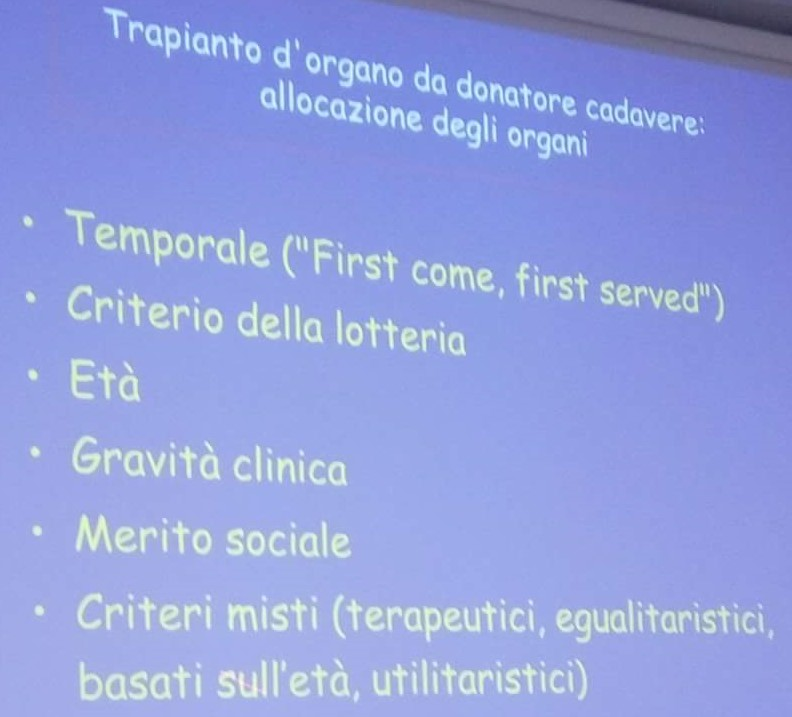
\includegraphics[width=2.98403in,height=1.96319in]{media/image15.jpeg}}{}}\label{section-7}

\subsection{I microrganismi sopravvivono mesi sulle superfici: MRSA, per
esempio, sopravvive sette mesi, enterococco per un
anno.}\label{i-microrganismi-sopravvivono-mesi-sulle-superfici-mrsa-per-esempio-sopravvive-sette-mesi-enterococco-per-un-anno.}

\subsection{\texorpdfstring{\protect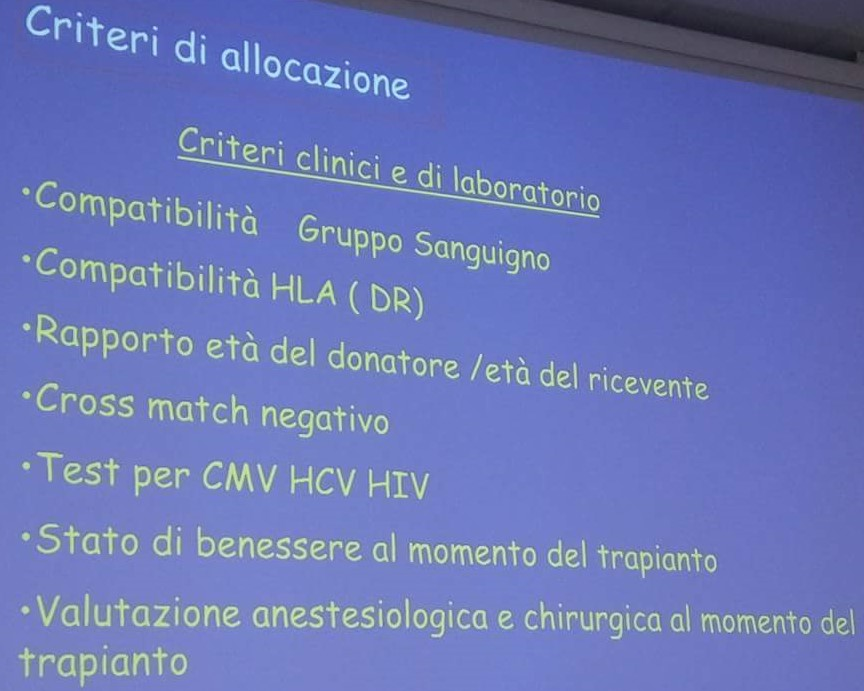
\includegraphics[width=3.24028in,height=1.85278in]{media/image16.jpeg}}{}}\label{section-8}

\subsection{Studi hanno dimostrato che l'adesione alla misura di igiene
delle mani è molto più alta dopo aver toccato il paziente, più bassa
dopo aver toccato le
superfici.}\label{studi-hanno-dimostrato-che-ladesione-alla-misura-di-igiene-delle-mani-uxe8-molto-piuxf9-alta-dopo-aver-toccato-il-paziente-piuxf9-bassa-dopo-aver-toccato-le-superfici.}

\subsection{\texorpdfstring{Un paziente che venga ammesso in una stanza
dove era stato precedentemente degente un paziente colonizzato o infetto
da un determinato microrganismo, ha un rischio più alto di acquisire
quel microrganismo: questo proprio perché le superfici rimangono
contaminate. C'è uno studio epidemiologico su un soggetto che ha
sviluppato un'infezione da \emph{Clostridium difficile} dove l'unico
fattore di rischio significativo era l'essere stato degente in una
stanza precedentemente occupata da un soggetto
infetto.}{Un paziente che venga ammesso in una stanza dove era stato precedentemente degente un paziente colonizzato o infetto da un determinato microrganismo, ha un rischio più alto di acquisire quel microrganismo: questo proprio perché le superfici rimangono contaminate. C'è uno studio epidemiologico su un soggetto che ha sviluppato un'infezione da Clostridium difficile dove l'unico fattore di rischio significativo era l'essere stato degente in una stanza precedentemente occupata da un soggetto infetto.}}\label{un-paziente-che-venga-ammesso-in-una-stanza-dove-era-stato-precedentemente-degente-un-paziente-colonizzato-o-infetto-da-un-determinato-microrganismo-ha-un-rischio-piuxf9-alto-di-acquisire-quel-microrganismo-questo-proprio-perchuxe9-le-superfici-rimangono-contaminate.-cuxe8-uno-studio-epidemiologico-su-un-soggetto-che-ha-sviluppato-uninfezione-da-clostridium-difficile-dove-lunico-fattore-di-rischio-significativo-era-lessere-stato-degente-in-una-stanza-precedentemente-occupata-da-un-soggetto-infetto.}

\subsection{\texorpdfstring{\protect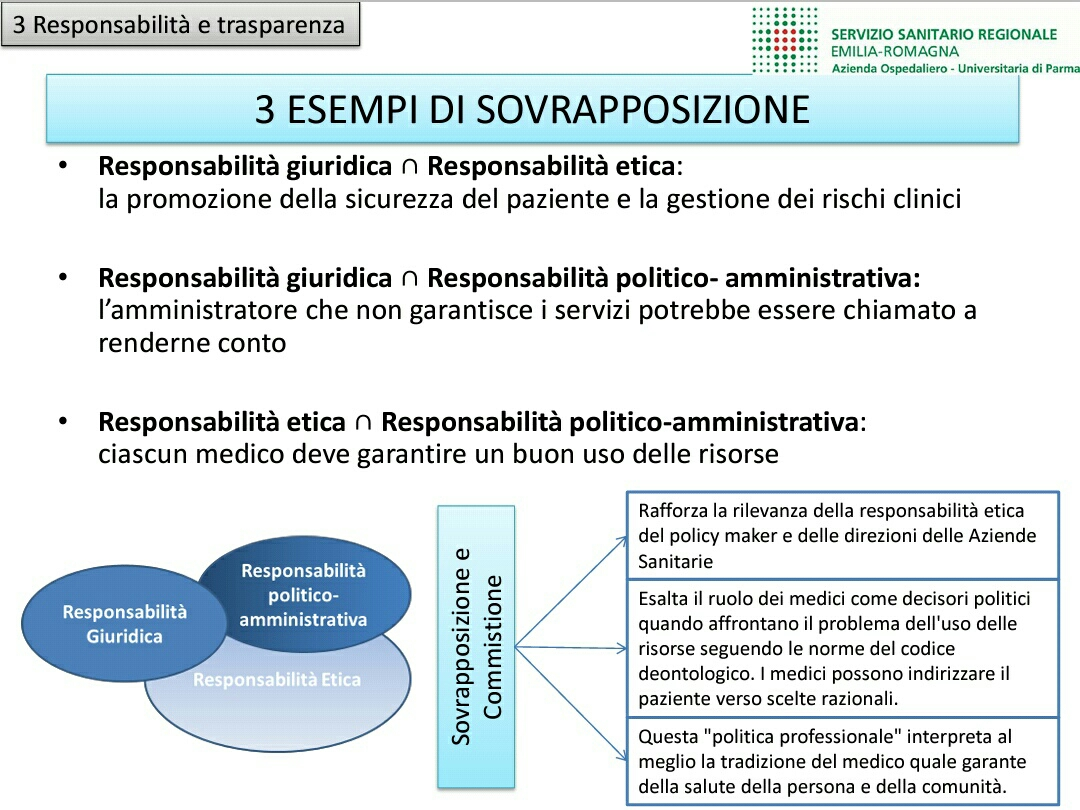
\includegraphics[width=4.63125in,height=2.94375in]{media/image17.jpeg}\protect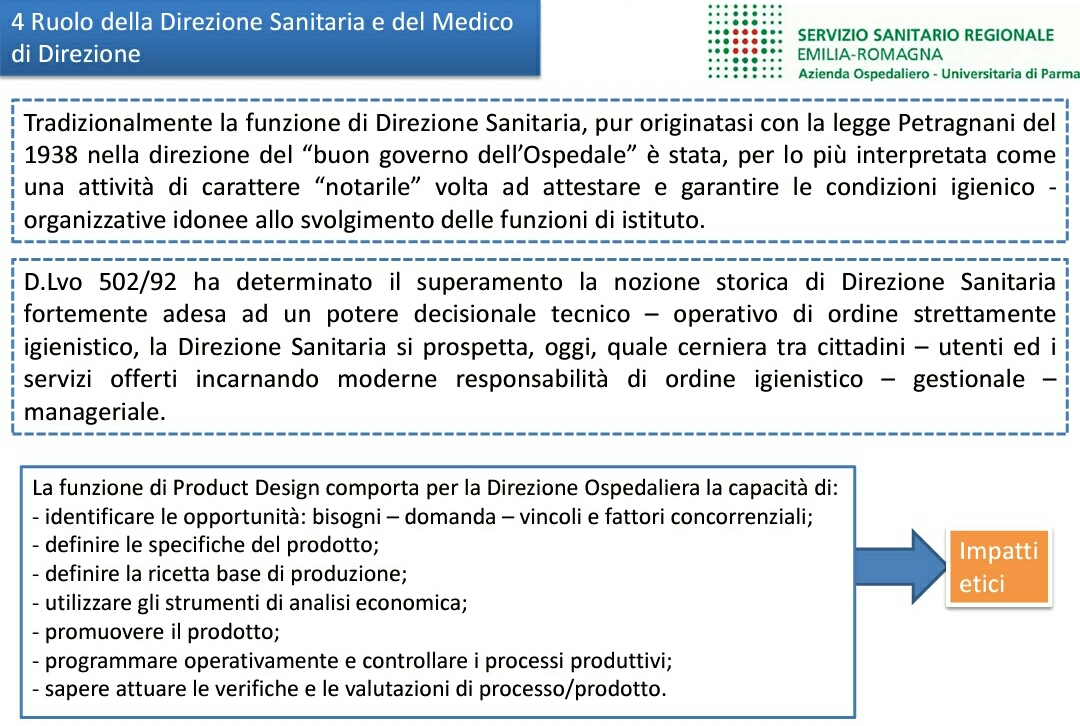
\includegraphics[width=2.44861in,height=3.03889in]{media/image18.jpeg}Infine
il rischio d'infezione aumenta all'aumentare della
contaminazione.}{Infine il rischio d'infezione aumenta all'aumentare della contaminazione.}}\label{infine-il-rischio-dinfezione-aumenta-allaumentare-della-contaminazione.}

\subsection{}\label{section-9}

\subsection{}\label{section-10}

\end{document}
